% Diese Zeile bitte -nicht- aendern.
\documentclass[course=erap]{aspdoc}

%%%%%%%%%%%%%%%%%%%%%%%%%%%%%%%%%
%% TODO: Ersetzen Sie in den folgenden Zeilen die entsprechenden -Texte-
%% mit den richtigen Werten.
\newcommand{\theGroup}{233} % Beispiel: 42
\newcommand{\theNumber}{A406} % Beispiel: A123
\author{Fikret Ardal \and Mert Corumlu \and Denis Paluca}
\date{Sommersemester 2021} % Beispiel: Wintersemester 2019/20
%%%%%%%%%%%%%%%%%%%%%%%%%%%%%%%%%
\DeclareMathOperator{\artanh}{artanh}
\usepackage{amssymb}
\usepackage{pgfplots}
\pgfplotsset{compat=newest}
\usepackage{parskip}

% Diese Zeile bitte -nicht- aendern.
\title{Gruppe \theGroup{} -- Abgabe zu Aufgabe \theNumber}
\graphicspath{{images/}}

\begin{document}
\maketitle

\section{Einleitung}

Die Entropie (engl.: Shannon entropy, sym.: $H$) ist in der Informationstheorie ein Maß für den mittleren Informationsgehalt einer Nachricht. Das Informationsgehalt (auch Überraschungswert gennant) eines Ereignisses nimmt mit zunehmenden Wahrscheinlichkeit des Ereignisses ab. Je unwahrscheinlicher das Ereignis ist, desto überraschender ist es, falls es geschieht. Formel für die Entropie eines Zufallsvariable $X$:

\begin{equation}
    \mathrm {H} (X)=-\sum _{i=1}^{n}{\mathrm {P} (x_{i})\log_2 \mathrm {P} (x_{i})}
\end{equation}

In der gegebenen Aufgabe geht es darum, die Entropie einer Zufallsvariable zu berechnen, gegeben sei die Wahrscheinlichkeitsverteilung der Zufallsvariable. Dafür muss man ein geeignetes Rahmenprogramm und die Entropiefunktion implementieren. Das Programm soll auf Genauigkeit und Performanz getestet.

Die Wahrscheinlichkeitsverteilung soll als Textdatei übergeben werden. Das Format ist wie folgt:

\begin{itemize}
    \item Die Datei enthält eine Liste von Zahlen
    \item Die Zahlen sind mittels Leerzeichen aufgeteilt
    \item Die Zahlen liegen zwischen 0 und 1 (inklusive)
    \item Die Summe der Zahlen ist gleich 1 (mit einer Fehlerspanne)
    \item Beispiel: 0.25 0.1 0.05 0.6
\end{itemize}

Die Datei wird von dem Rahmenprogramm, das in C programmiert ist, eingelesen. Die eingelesene Zahlen werden in ein Array mit
Fließkommazahlen gespeichert und als Pointer dem Assemblerprogramm übergeben. Das Assemblerprogramm berechnet die Entropie, und danach gibt das Rahmenprogramm die Entropie aus. Die Performanz und die Genauigkeit der Implementierung werden mittels Vergleich zwischen eine Basisimplementierung und verschiedene Implementierungen festgestellt.

In folgenden Abschnitten wird der Lösungsansatz genauer erläutert. Ins besonders fokussieren wir an der Logarithmusfunktion und an die angewendete Techniken zur SIMD-Vektorisierung der Entropiefunktion. Danach besprechen wir die Genauigkeit und Performanz verschiedene Implementierungen, und welche Art von Trade-offs sie eingehen. Wir schließen die Arbeit mit einer kurzen Zusammenfassung unserer Ergebnisse sowie mit einigen abschließenden Gedanken über mögliche zukünftige Entwicklungen.

\section{Lösungsansatz}
Bei der Berechnung der Entropie ist der zeitaufwendigste Teil im Code die Berechnung des Logarithmus.
% Daher haben wir zunächst beschlossen, die Anzahl der Logarithmusoperationen auf ein Minimum zu reduzieren, indem wir die Entropiefunktion (1) in eine riesige Logarithmusform bringen:
% \begin{equation*}
%         \text {Sei } X = \{x_{1},x_{2}, \cdots, x_{n}\}
% \end{equation*}
% \begin{equation*}
%     \mathrm {H} (X)= - \log_2 (\mathrm{P}(X=x_{1})^{\mathrm{P}(X=x_{1})} \cdot \mathrm{P}(X=x_{2})^{\mathrm{P}(X=x_{2})} \cdots \mathrm{P}(X=x_{n})^{\mathrm{P}(X=x_{n})})
% \end{equation*}
% Aber wir haben festgestellt, dass die Potenzfunktion mehr kostet als die Logarithmusfunktion, deshalb haben wir beschlossen, die Logarithmusfunktion für jede Wahrscheinlichkeit zu berechnen. \newline
Zur Berechnung der Logarithmusfunktion gibt es drei Hauptmethoden:
\begin{itemize}
    \item Approximation als Polynom
    \item Lookup Tabelle
    \item Approximation mit Hilfe von Lookup Tabelle (glibc Methode).
\end{itemize} 

Da wir mehrere Logarithmusfunktionen ausprobieren möchten, haben wir die Signatur der Entropiefunktion entsprechend erweitert. Man soll jetzt auch den Pointer der Logarithmusfunktion angeben.

Die Entropiefunktion an sich ist auch nicht direkt implementiert, wie von der Gleichung spezifiziert, sondern es nutzt die Kahan-Summe-Algorithmus.~\cite{kahan} Die Kahan-Summe hilft die Auslöschung bei einer Reihe von Additionen zu vermeiden.

\subsection{Approximation}
Der erste Ansatz an dieses Problem war, eine Polynomdarstellung der Logarithmusfunktion zu finden, die nicht aufwendig zu berechnen ist und auch für kleine Werte von $x$ schnell genug konvergiert.

Nach dem Testen einiger Möglichkeiten haben wir uns für zwei verschiedene Methoden zur Approximation der Logarithmusfunktion entschieden. Diese Methoden sollen leistungsfähig, präzise und vektorisierbar sein.

Da jede Gleitkommazahl die Form $x = 2^{k} \cdot z$ für ein $k \in \mathbb{Z}$ und $ z \in \mathbb{Q}$ hat, können wir zuerst den Exponenten extrahieren und dann Logarithmus für $z$ berechnen die zwischen $1$ und $2$ liegt.
\[\log_2{x} = k + \frac{\ln{z}}{\ln{2}}\]
Bei den folgenden Approximierungsmethoden haben wir immer berücksichtigt, wie anpassungsfähig diese Methoden an die SIMD-Version sind, was für den Performance-Gewinn eine große Rolle spielen wird.

\subsubsection{ARTANH Approximation}
Wir können $\ln(x)$ als eine  konvergente Summe von Potenzreihen schreiben, indem wir die Taylorreihe von $\artanh$ verwenden. Die Partialsumme der Potenzreihe konvergiert für kleine Werte von $x$ schneller als die normale Taylorreihe von $\ln(x)$.
\begin{equation}
    \ln(x) = 2 \cdot \artanh\left(\frac{x-1}{x+1}\right) = 2\left(\sum _{k=0}^{\infty}{\frac{1}{2k+1} \cdot \left(\frac{x-1}{x+1}\right)^{2k+1}}\right)
\end{equation}

\begin{equation}
   \text{Sei }  S_{n} = 2\left(\sum _{k=0}^{n}{\frac{1}{2k+1} \cdot \left(\frac{x-1}{x+1}\right)^{2k+1}}\right)
   \label{eq:artanh}
\end{equation}

Obwohl die Artanh-Approximation eine Division erfordert, ist der absolute Unterschied zwischen Logarithmusfunktion und Artanh-Approximation mit $S_{2}$ fast $0$, wenn die Zahl zwischen $1$ und $2$ liegt.

\subsubsection{Remez Algorithmus}
Der Remez-Algorithmus ist ein Minimax-Approximations-Algorithmus, das die maximale absolute Differenz zwischen dem Polynom und der gegebenen stetigen Funktion im Intervall $[a,b]$ minimiert ~\cite{remez}.

Um Polynome zur Approximation von $\ln(x)$ im Intervall $[1,2)$ zu erzeugen, haben wir ein Open-Source-Projekt namens „lolremez“~\cite{lolremez} verwendet.
Wir haben 2 verschiedene Polynome mit dem Grad $2$ und $4$ implementiert.

\begin{equation}
    \mathrm{P_{2}}(z) = -0.344845 \cdot z^{2}+ 2.024658 \cdot z -1.674873
    \label{eq:deg2}
\end{equation}

\begin{equation}
    \mathrm{P_{4}}(z) = -0.081616z^{4} + 0.645142z^{3} -2.120675z^{2} + 4.070091z -2.512854
    \label{eq:deg4}
\end{equation}

Das Polynom mit Grad $2$ liefert ungenauere Ergebnisse, gewinnt aber auch etwas an potenzieller Geschwindigkeit, da es $2$ Multiplikationen weniger hat.

\subsection{Lookup Tabelle }
Ein anderer Ansatz besteht darin, eine sogenannte Lookup Tabelle zu benutzen. Anstatt dass wir der in Mantisse gespeicherte Wert zu $log_2(x)$ annähern, speichern wir vorher diese Werte in einer Tabelle und geben sie zurück gemäß der Mantisse. Für das Erhalten der Genauigkeit von $100\%$ brauchen wir insgesamt $2^{23}$ Einträge in der Tabelle, welche aber nämlich 
\[2^{23} . 4 \text{ bytes } = 2^{15} \text{ Kb } = 32 \text{ Mb }\]

Unter Berücksichtigung das Experiment von der Universität Berkeley ~\cite{fast_log} haben wir uns entschieden, nur erste $16$ bits von der Mantisse für die Tabelle zu benutzen und die letzten $7$ bits zu ignorieren.

\begin{figure}[h]
    \centering
    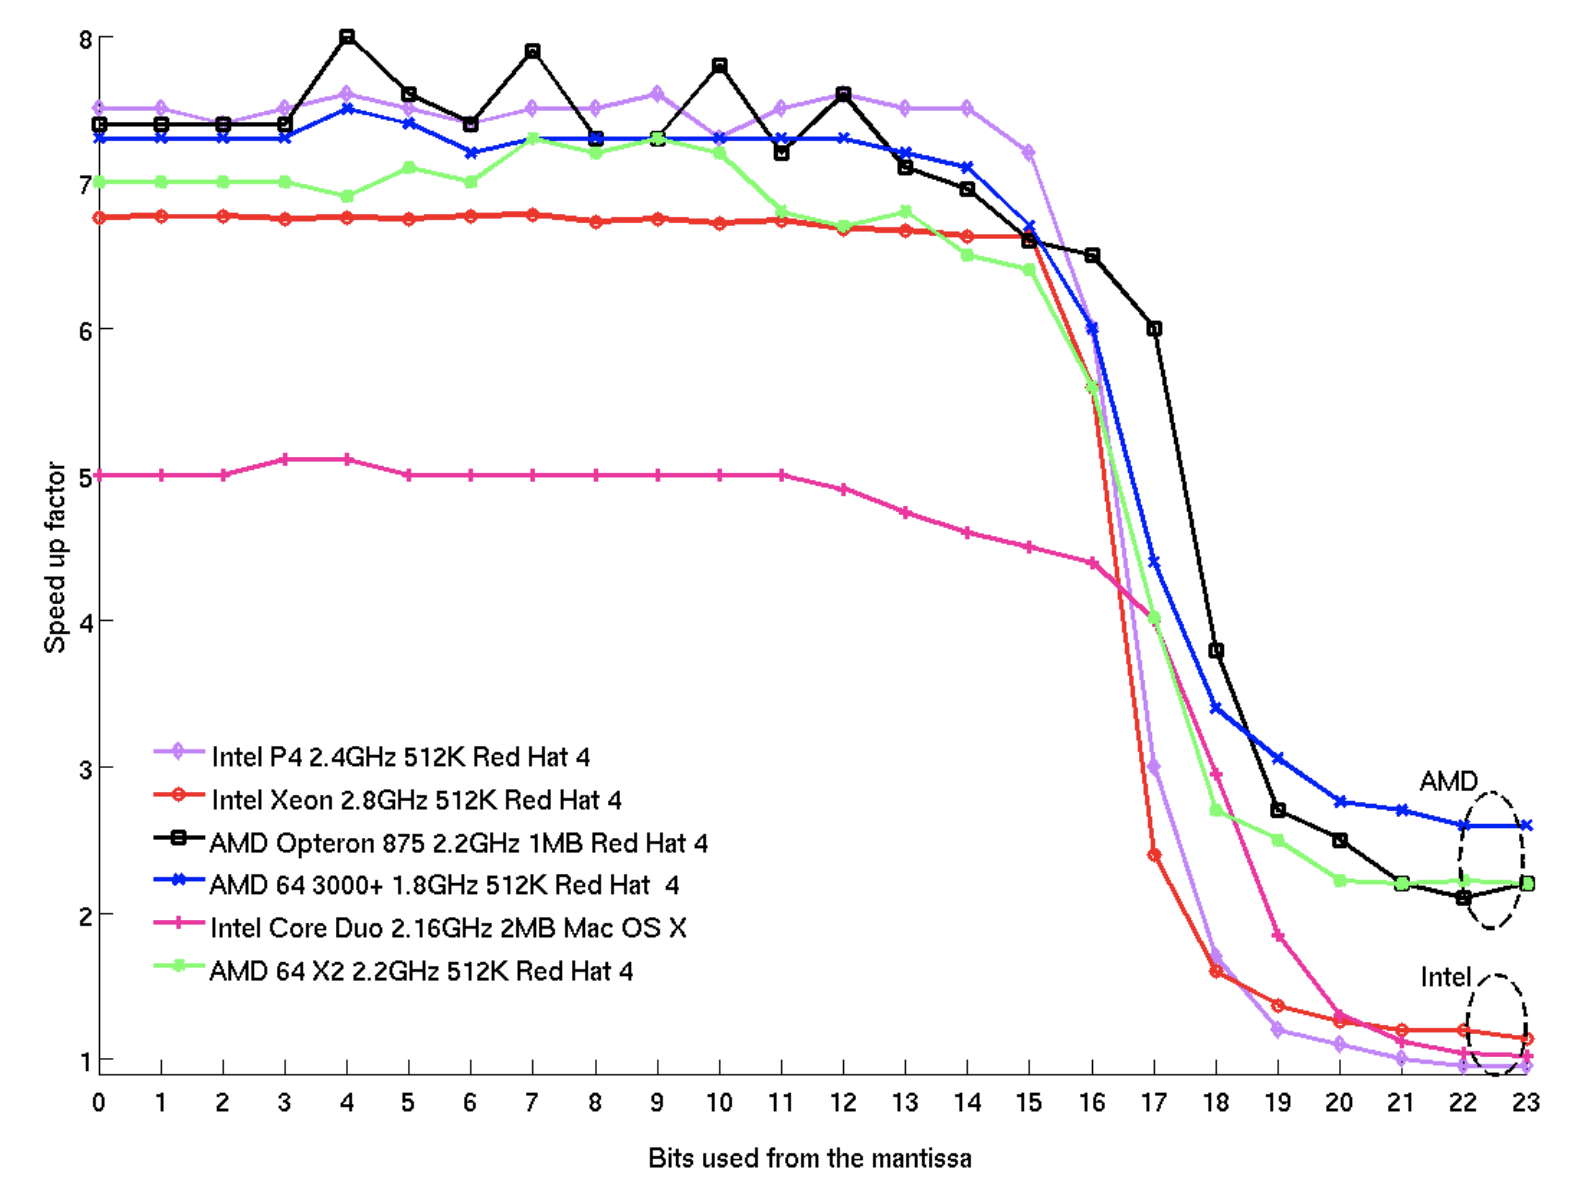
\includegraphics[scale=0.35]{lookup_berkeley.png}
    \caption{Performanz-Genauigkeit Trade-Off der logf mit Lookup Tabelle auf unterschiedliche Systeme}
    \label{graph:lookup_berkeley}
\end{figure}

Weil wir die Tabelle somit verkleinert haben, können wir die Cache effizienter benutzen um Performanz zu erhöhen, jedoch verlieren wir die Genauigkeit im Durchschnitt um $6.55 \cdot 10^{-6}$. Das ist einer der Trade-Offs, die wir während der Entwicklung begegnet und sie werden in folgender Abschnitte eingegangen.
 
\subsection{Glibc - log2f}
Die glibc Implementierung von $log2f$ nutzt eine Kombination von Approximation und Lookup Tabelle. Erst ist x in Mantisse $z$ und Exponent $k$ geteilt.

\[log_2(x) = log_2(2^k \cdot z) = k + log_2(z) \]

Mittels z ist ein Index berechnet, mit dem man in der Lookup-Tabelle eine Variable c ($\approx z$) und $log_2(c)$ findet.

\[log_2(x) = k + log_2(z/c) + log_2(c)\]

Jetzt muss man nur $log_2(\frac{z}{c})$ berechnen, das wird durch die Taylor-Reihe approximiert. Das liefert genaue Ergebnisse, weil $\frac{z}{c}$ sehr nähe zu $1$ ist, wo die Taylor-Reihe sehr schnell konvergiert. 

% Die glibc Implementierung von $log2f$ nutzt eine Kombinitaion von Approximation und Lookup Tabelle. Erst wird die Zahl $x$ in Form $2^k\cdot z$ gebracht, wo $k \in \mathbb{Z}$ und $\ln2 \leq z \leq 2\cdot\ln2$. Dann wird diese Interval in $16$ Subintervals geteilt. 

% Mittels $z$ kann man berechnen, in welcher Subinterval $z$ liegt. Der Mittelpunk dieser Subinterval ist $c$. Die Werte $\frac{1}{c}$ und $\log_2(c)$ in der Tabelle gespeichert. Außerdem wird die Taylor Series von Grad $4$ benutzt, um $f(x) = \log_2(x + 1)$ zu approximieren. Jetzt ist es zu berechnen: \[\log_2(x) = f(\frac{z}{c} - 1) + \log_2(c) + k\]

% Weil die Zahl $\frac{z}{c} - 1 \approx 0$, konvergiert Taylor Series sehr schnell und liefert $log2f$ ein sehr präzises Ergebnis.

\subsection{SIMD}
Für unsere Algorithmen sind Optimierungen durch SIMD deutlich möglich und sinnvoll. SIMD-Befehle nutzen XMM Registern, die $128$ Bits haben. Unsere Algorithmen arbeiten mit Fließkommazahlen, die $32$ Bits haben. Daher können wir mittels SIMD-Befehle $4$ Einträge gleichzeitig bearbeiten. Dadurch kann man ein theoretischen maximalen Speedup von $4$ erreichen.

% Um unnötige Überprüfungen in unsere SIMD-Implmentation zu vermeiden, erweitern wir das Array der Fließkommazahlen, sodass die Länge durch 4 trennbar ist. Die zusätzliche Zahlen sind alle $0$ und sie verändern nicht das Endergebnis. Außerdem allozieren wir das Array 16-Byte-Aligned, dann können wir Befehle, wie z.B. \emph{movaps}, nutzen, die effizienter sind als ihre unaligned Gegenstücke.

% Der SIMD Entropie Algorithmus funktioniert wie folgt:
% \begin{enumerate}
%     \item In einem XMM-Register, SUM, sind 4 Fließkommazahlen geladen, die gleich 0 sind.
%     \item In eine Schleife von 0 bis n-1 mit Schrittweite 4, sind 4 Einträge von das Array gelesen.
%     \item Der Logarithmus der Einträge ist berechnet und mit den Einträgen multipliziert.
%     \item Die Werte der Multiplikation sind dann auf dem Register SUM subtrahiert.
%     \item Nach der Schleife, sind die Einträge der Register SUM horizontal addiert und zurückgegeben.
% \end{enumerate}

Natürlich sind die Logarithmusfunktionen ebenfalls vektorisiert. Hier wird einer der größten Vorteile der Verwendung von Approximationen deutlich. Die Approximationsfunktionen verwenden nur eine Reihe von sehr einfachen Operationen, wie z.B. Addition, Multiplikation, Bitverschiebung und so weiter. Diese Operationen sind in SIMD mit wenig bis gar keinem Overhead replizierbar. Daher ist es möglich, sich dem maximalen Speedup anzunähern.

Im Gegensatz dazu ist die Vektorisierung von der Lookup-Version unsere Logarithmusfunktion deutlich ineffizienter. Den Index zu finden für jeden Eintrag, kann man noch gut vektorisieren. Mit 2 Befehle findet man das Index von alle 4 Einträge. Nachdem man die Indices hat, muss man jeden Eintrag der Lookup-Tabelle einzeln in das Register laden. Da diese Einträge in der Lookup-Tabelle höchstwahrscheinlich weit voneinander entfernt sind, fallen viele Cache-Misses an. 

\subsection{Umgang mit denormalen Zaheln}
Um die oben beschriebenen Methoden an die denormalen Zahlen anzupassen ist eine spezielle Behandlung benötigt. Unsere Methoden funktionieren für die Zahlen $x = 2^k \cdot z$ wo $1 \leq z < 2$. Bei den denormalizierten Zahlen liegt $z$ im Interval $[0,1)$, wo unsere Approximationen sehr ungenau sind. Deswegen müssen die denormalen Zahlen erst normaliziert werden. 

Dafür multiplizieren wir die Zahlen mit $2^{23}$, deren Exponent gleich $0$ ist. Unsere Zahl ist damit normaliziert, aber ist jetzt $2^{23}$ mal mehr als wir erwarten würden. \[log_2(x\cdot 2^{23}) = log_2(x) - log_2(2^{23}) = log_2(y) - 23\]
Aus diesem Grund subtrahieren wir $23$ von dem Exponent und führen wir die normalen Schritte für die Logarithmusfunktion.

% Für SIMD ist der Ansatz gleich, aber die Methode ändert sich denn ein Vergleich für einzelne Zahlen ist nicht mehr möglich. Wohingegen werden die normalen Zahlen mit $1.0$ und denormalen Zahlen mit $2^{23}$ multipliziert und von deren Exponent 23 subtrahiert. Die Bitmasken dafür sehen wie folgt aus:

% \[
% \begin{array}{ccc}
%      1.0f & : & 0\;01111111\;00000000000000000000000  \\
%     2^{23}f & : & 0\;10010110\;00000000000000000000000 \\
%     \text{xor Maske}: & : & 0\;11101001\;00000000000000000000000
% \end{array}
% \]

% Die Masken aus $pcmpeqd$ mit $0$ werden erst mit xor-Masken andet, dann wird das Ergebnis mit $1.0f$ xored. Die Resultat ist $1.0f$ für normalizierte Zahlen und $2^{23}$ für denormale Zahlen.
% Am Ende wird die zu logierende Zahlen mit diesem Ergebnis multipliziert.

% \subsection{Glibc (just draft for us)}
% \[x = 2^k . z\] where \[ln2 \leq z < 2ln2\]

% \[log1p(x) = \ln{x + 1}\]

% with

% \[log1p(\frac{z}{c} - 1) + log_2(c) = \ln{(\frac{z}{c})}+ log_2(c) = \ln{(z)}\]

% then

% \[log_2(x) = \frac{\ln{(\frac{z}{c})}+ log_2(c)}{\ln2} + k\]

% to approximate $\ln(x + 1)$ they use Taylor Series of 4th degree.

% So we need to figure out what is c, because $\frac{z}{c}$ is a number which is really close to 1
\section{Genauigkeit}
Die Genauigkeit des Programms ist stark abhängig von der Genauigkeit unsere log2-Implementierung. Für die log2-Approximationen können wir für die Genauigkeit eine analytische Untersuchung durchführen. Wir sind auf die Differenz zwischen log2 und unseren Approximationen der log2 interessiert. Dann finden wir die Ableitung der Differenz, um das Maximum/Minimum im Bereich von 1 bis 2 herauszuziehen.  

\subsubsection*{Log2 Approx DEG2 -- $P_{2}(x)$ \eqref{eq:deg2}}

\begin{equation*}
    (\mathrm{log_{2}}(x) - \mathrm{P_{2}}(x))'
    = \frac{1}{x \cdot \ln(2)} + 0.68969 \cdot x - 2.024658
\end{equation*} \par

Nullstellen: $x_{1} \approx 1.718089, x_{2} \approx 1.217517$ \par

Der größte absolute Fehler für diese Approximation ist ungefähr $4.941 \cdot 10^{-3}$.

\subsubsection*{Log2 Approx DEG4 -- $P_{4}(x)$ \eqref{eq:deg4}}

\begin{equation*}
    (\mathrm{log_{2}}(x) - \mathrm{P_{4}}(x))'
    = \frac{1}{x \cdot \ln(2)} + 0.32646 \cdot x^{3}
    - 1.93543 \cdot x^{2} +4.24135 \cdot x - 4.07009
\end{equation*} \par

Nullstellen: $x_{1} \approx 1.08506,  x_{2} \approx 1.31912, x_{3} \approx 1.62916, x_{4} \approx 1.89513$ \par

Der größte absolute Fehler für diese Approximation ist ungefähr. $8.752644 \cdot 10^{-5}$.

\subsubsection*{Log2 Approx ARTANH -- $S_{2}(x)$ \eqref{eq:artanh}}

\begin{equation*}
    (\mathrm{log_{2}}(x) - \mathrm{S_{2}}(x) \cdot \frac{1}{ln(2)})'
    = \dfrac{x^6-6x^5+15x^4-20x^3+15x^2-6x+1}{\ln\left(2\right)x\left(x+1\right)^6}
\end{equation*} \par

Nullstellen: $x = 1$ \par

Auf die Stelle x gleich 1 ist die Differenz 0. Aber, der größte Wert im Bereich findet sich auf die Stelle x = 2, weil der Funktion steigend ist. Der größte absolute Fehler für diese Approximation ist ungefähr $2,063996 \cdot 10^{-4}$.

\begin{figure}[h]
  \centering
  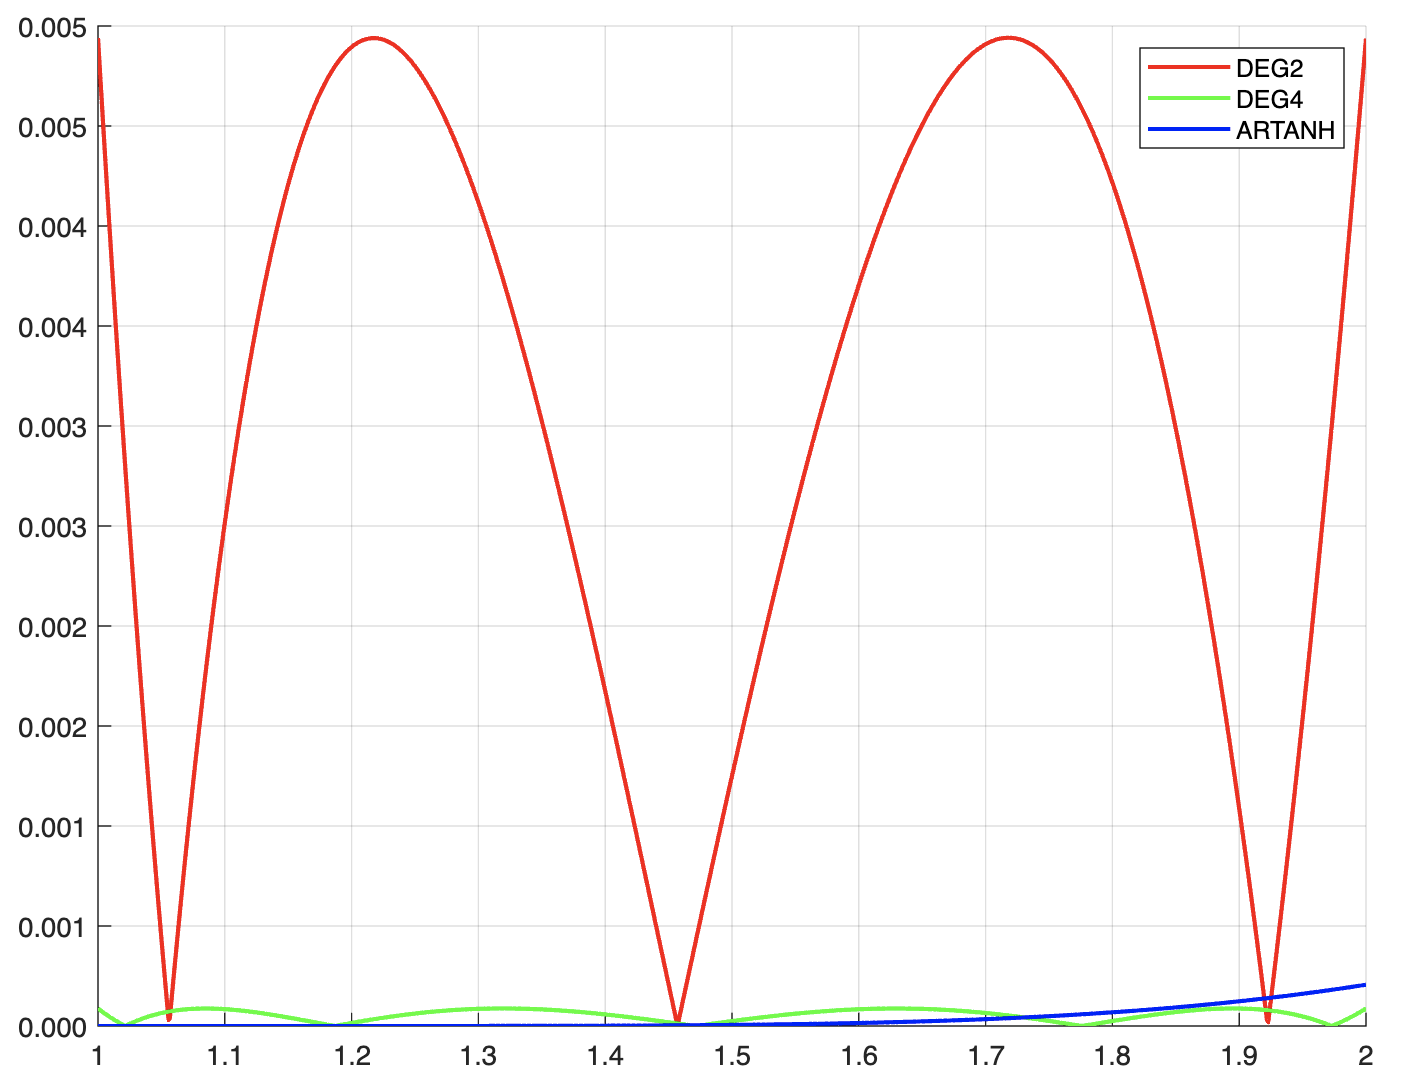
\includegraphics[scale=0.35]{abs_mistake.png}
  \caption{Absolute Fehler der Logarithmusfunktionen im $[1,2)$}
    \label{fig:absolute-mistake}
\end{figure}

Wir erwarten, dass die DEG4-Approximation uns bessere Ergebnisse liefert, weil es den kleinsten Fehler hat. (Siehe Abbildung \ref{fig:absolute-mistake})

Wir haben nur den maximalen absoluten Fehler für die log2 im Bereich [1,2] berechnet. Am Ende wird der Fehler für die log2 Approximation noch kleiner, weil diese Zahl mit dem log2 vom Exponenten addiert wird. Der log2 des Exponenten ist im Intervall [-126,0] und der log2 der Mantisse ist im Intervall [0,1]. Daher sinkt der relative Fehler mit der Addition. Der Fehler für die Lookup Version der log2 mit der empfohlene 16-Bit-Mantisse ist $6.55 \cdot 10^{-6}$.~\cite{fast_log}
% Der absolute Fehler sinkt auch (in Vergleich zu andere 32 Bit Fließkommaberechnung), weil bei der Addition Rundungsfehler auftritt, und das kann potenziell falsch berechnete Stellen der log2 der Mantisse entfernen. \\


Die Berechnung der Entropiefunktion enthält eine Multiplikation von der Logarithmusfunktion mit einem Wert $x$, der immer kleiner gleich 1 ist, welches die Abnahme des absoluten Fehlers verursacht.

Bei einer naiven Implementierung der Entropiefunktion gibt es auch einen Unterschied in Genauigkeit zwischen der Skalar- und SIMD-Version der Entropie. Wobei der SIMD Version genauer ist. Da der SIMD Version 4 Teil-summen berechnet, werden weniger Additionen von Rundungsfehler beeinflusst. Immer noch haben wir bemerkt, dass in beiden Fällen unsere Ergebnisse sehr stark von Rundungsfehler beeinflusst wurden.

\begin{figure}[h]
\centering
\begin{tikzpicture}
    \begin{axis}[
        symbolic x coords={log2f, DEG2, DEG4, ARTANH, Lookup},
        xtick=data,
        ymode = log,
        width = \textwidth *0.65
      ]
        \addplot[ybar] coordinates {
            (log2f,   0.000010)
            (DEG2,  0.000671)
            (DEG4,   0.000013)
            (ARTANH, 0.0000275) 
            (Lookup, 0.000010)
        };
    \end{axis}
\end{tikzpicture}
\caption{Entropiefehler Größenordnung (Durchschnitt bei zufälligen Daten)}
\end{figure}

Wie schon erwähnt in dem Ansatz, nutzen wir die Kahan-Summe~\cite{kahan}, um Rundungsfehler zu vermeiden. Die Kahan-Summe speichert der unbehandelte Teil  einer Addition in die Variable Kompensation und bei der nächste Addition wird die Kompensation aufaddiert. Die Kahan-Summe nimmt an, dass die Summe größer als der nächste zu addierende Zahl ist. Diese Annahme gilt bei uns auch. Wenn wir die Kahan-Summe verwenden sind die Ergebnisse bei SIMD und Skalar fast gleich.
\section{Performanzanalyse}
Die Performanz der Entropiefunktion hängt von vielen Faktoren ab. Wir wenden trotzdem einige Optimierungen an, die in der Theorie die Performanz verbessern sollen. In dieser Abschnitt geht es darum, wie unsere Optimierungen auf die Performanz auswirkt.

Die erste Optimierung liegt an SIMD Prinzip. Die Entropiefunktion lässt sich sehr einfach vektorisieren, außer der Verwendung von log2f-glibc und der Lookup-Tabelle.

Um unnötige Überprüfungen in unsere SIMD-Implmentation zu vermeiden, erweitern wir das Array der Fließkommazahlen, sodass die Länge durch 4 trennbar ist. Die zusätzliche Zahlen sind alle $0$ und sie verändern nicht das Endergebnis. Außerdem allozieren wir das Array 16-Byte-Aligned, dann können wir Befehle, wie z.B. \emph{movaps}, nutzen, die effizienter sind als ihre unaligned Gegenstücke.

% can be removed
Wir speichern die Konstanten für die Remez und Artanh Approximations im Speicher in der Reihenfolge der Verwendung. Das führt zu schnelleren Speciherzugriffen, weil dann die Konstanten in Cache geladen und von der Cache gelesen werden können.

% Eine andere Optimierung ist Software-Pipelining in Logarithmusfunktionen. Wir versuchen die Pipeline so zu unterstützen, dass die unabhängigen arithmetischen Operationen einander nicht blockieren. Assembly Implementation lässt der Pipelining besser helfen.

In allen Implementationen behandeln wir die Spezialfälle nicht, nämlich NaN, $\pm$Inf, $\pm$0 und negative Zahlen nicht. Der Grund ist wir stellen uns in der Entropiefunktion sicher, dass in die Log-Funktion eingegebener Wert immer im Interval $[0,1]$ liegt. Wenn der Wert $0$ ist, spielt das Ergebnis von der Log-Funkiton keine Rolle denn es wird später mit $0$ multipliziert. Damit sparen wir einige Branches in der Funktion, was gut auf die Performanz wirkt.

Unsere Logartihmusfunktionen sind stark für Entropieberechnung spezialisiert. Dazu lassen wir in der Assembly Implementation einige ABI Konventionen aus. Wir sichern Caller-Saved Registern in Entropiefunktion nicht denn wir wissen genau welche Registern in der Log-Funktion geändert wird. Dies erlaubt einen bemerkenswerten Gewinn an der Performanz.

\begin{figure}[h]
    \centering
    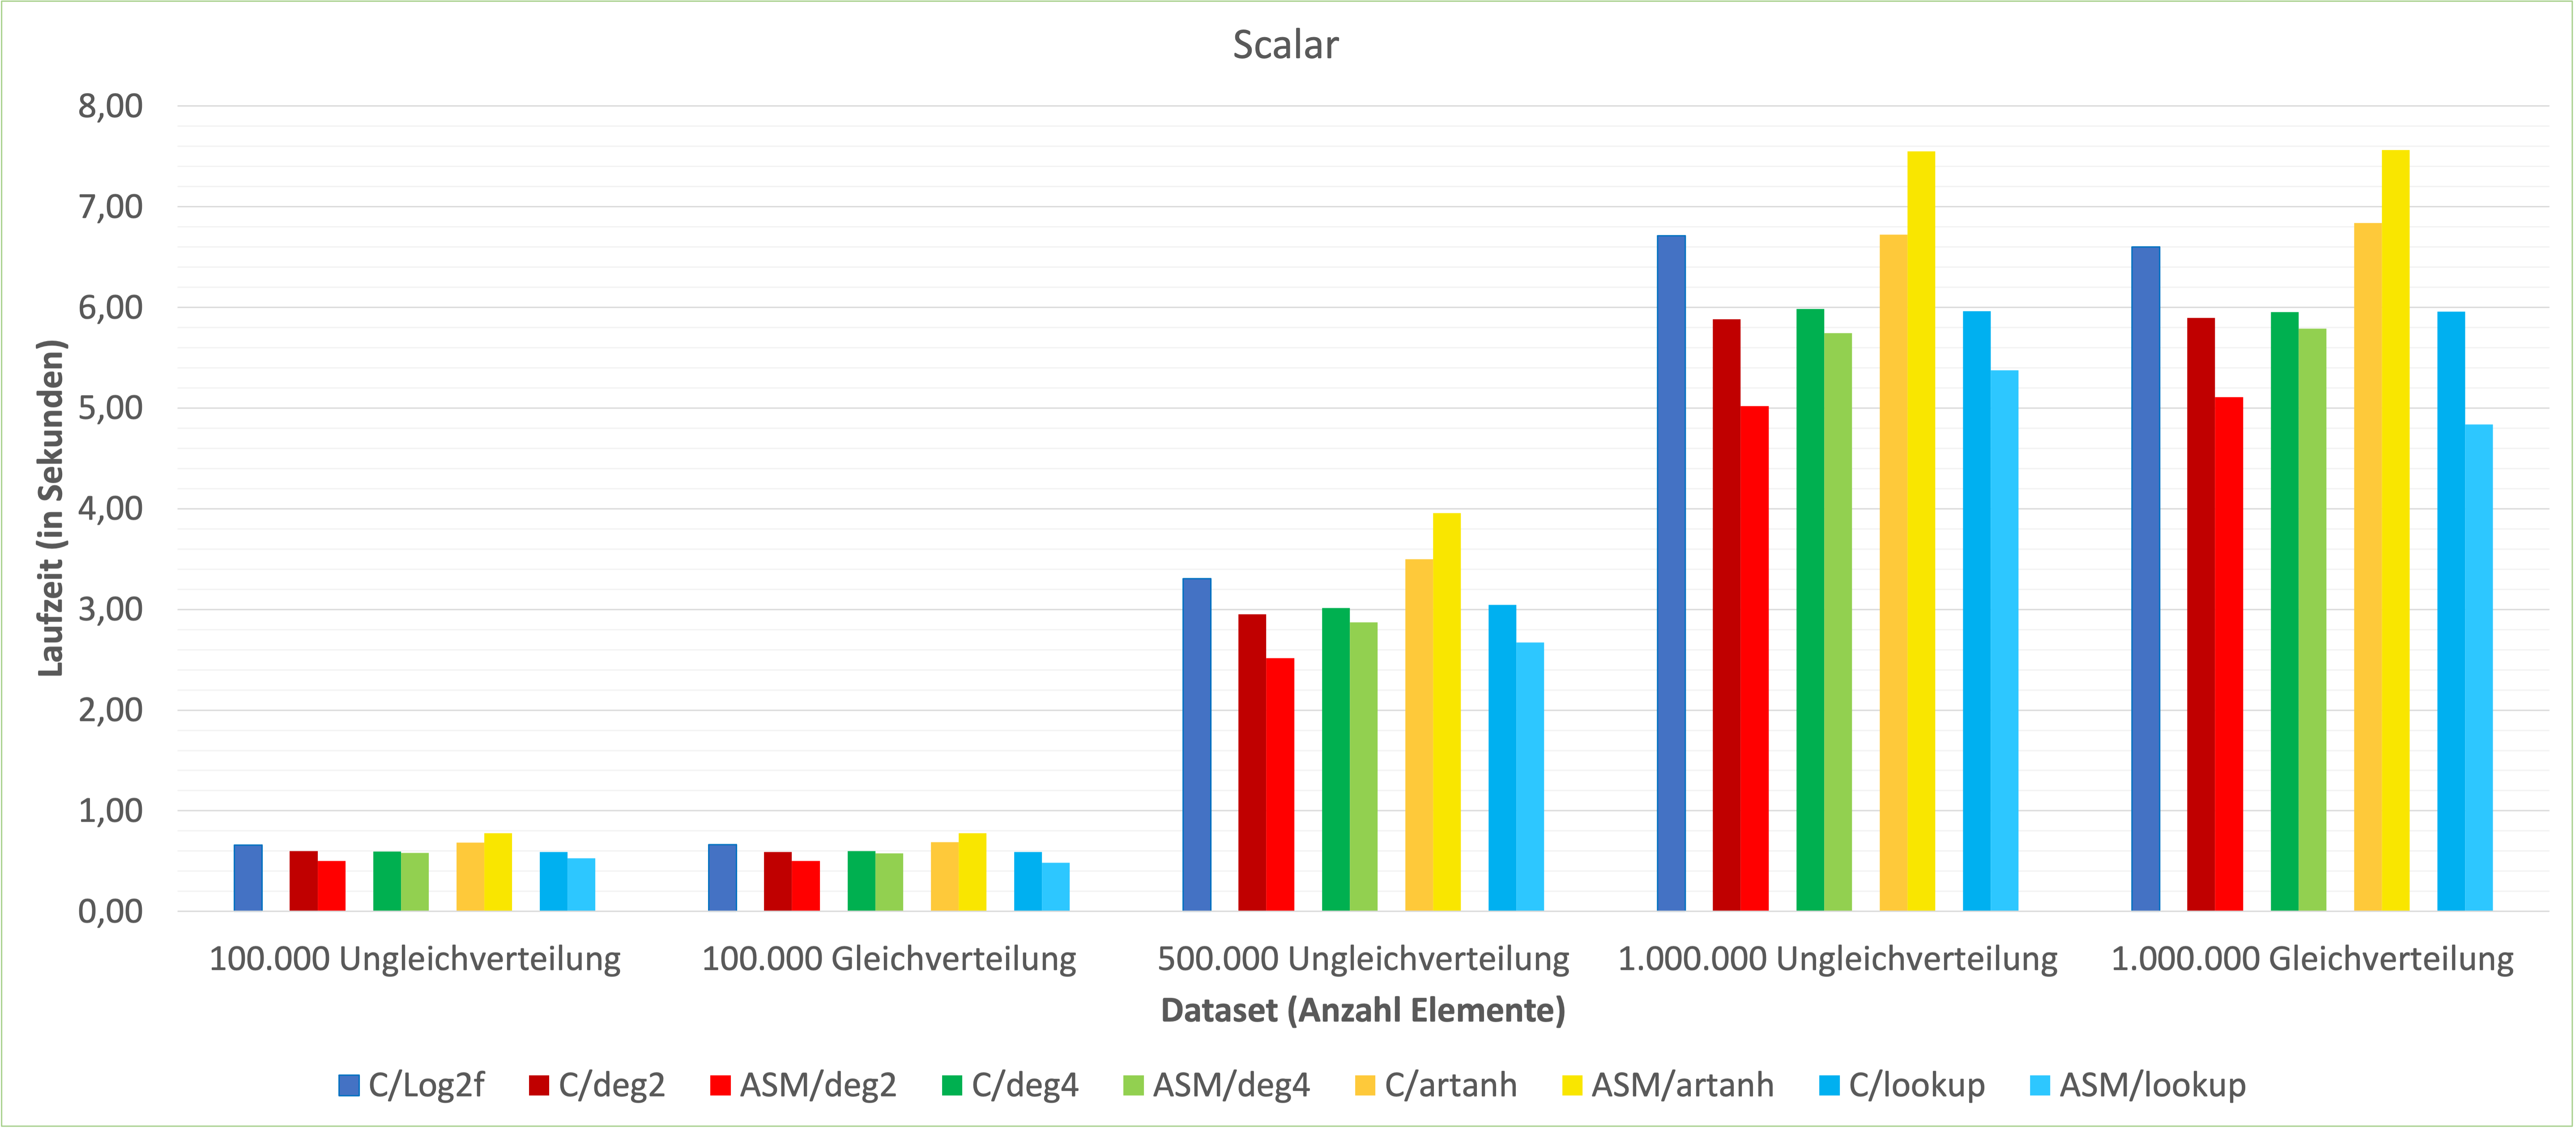
\includegraphics[scale=0.3]{graph_scalar.png}
    \caption{Performazgrafik zu skalarer Implementation mit 1000 Iterationen}
    \label{fig:graph_scalar}
\end{figure}

\begin{figure}[h]
    \centering
    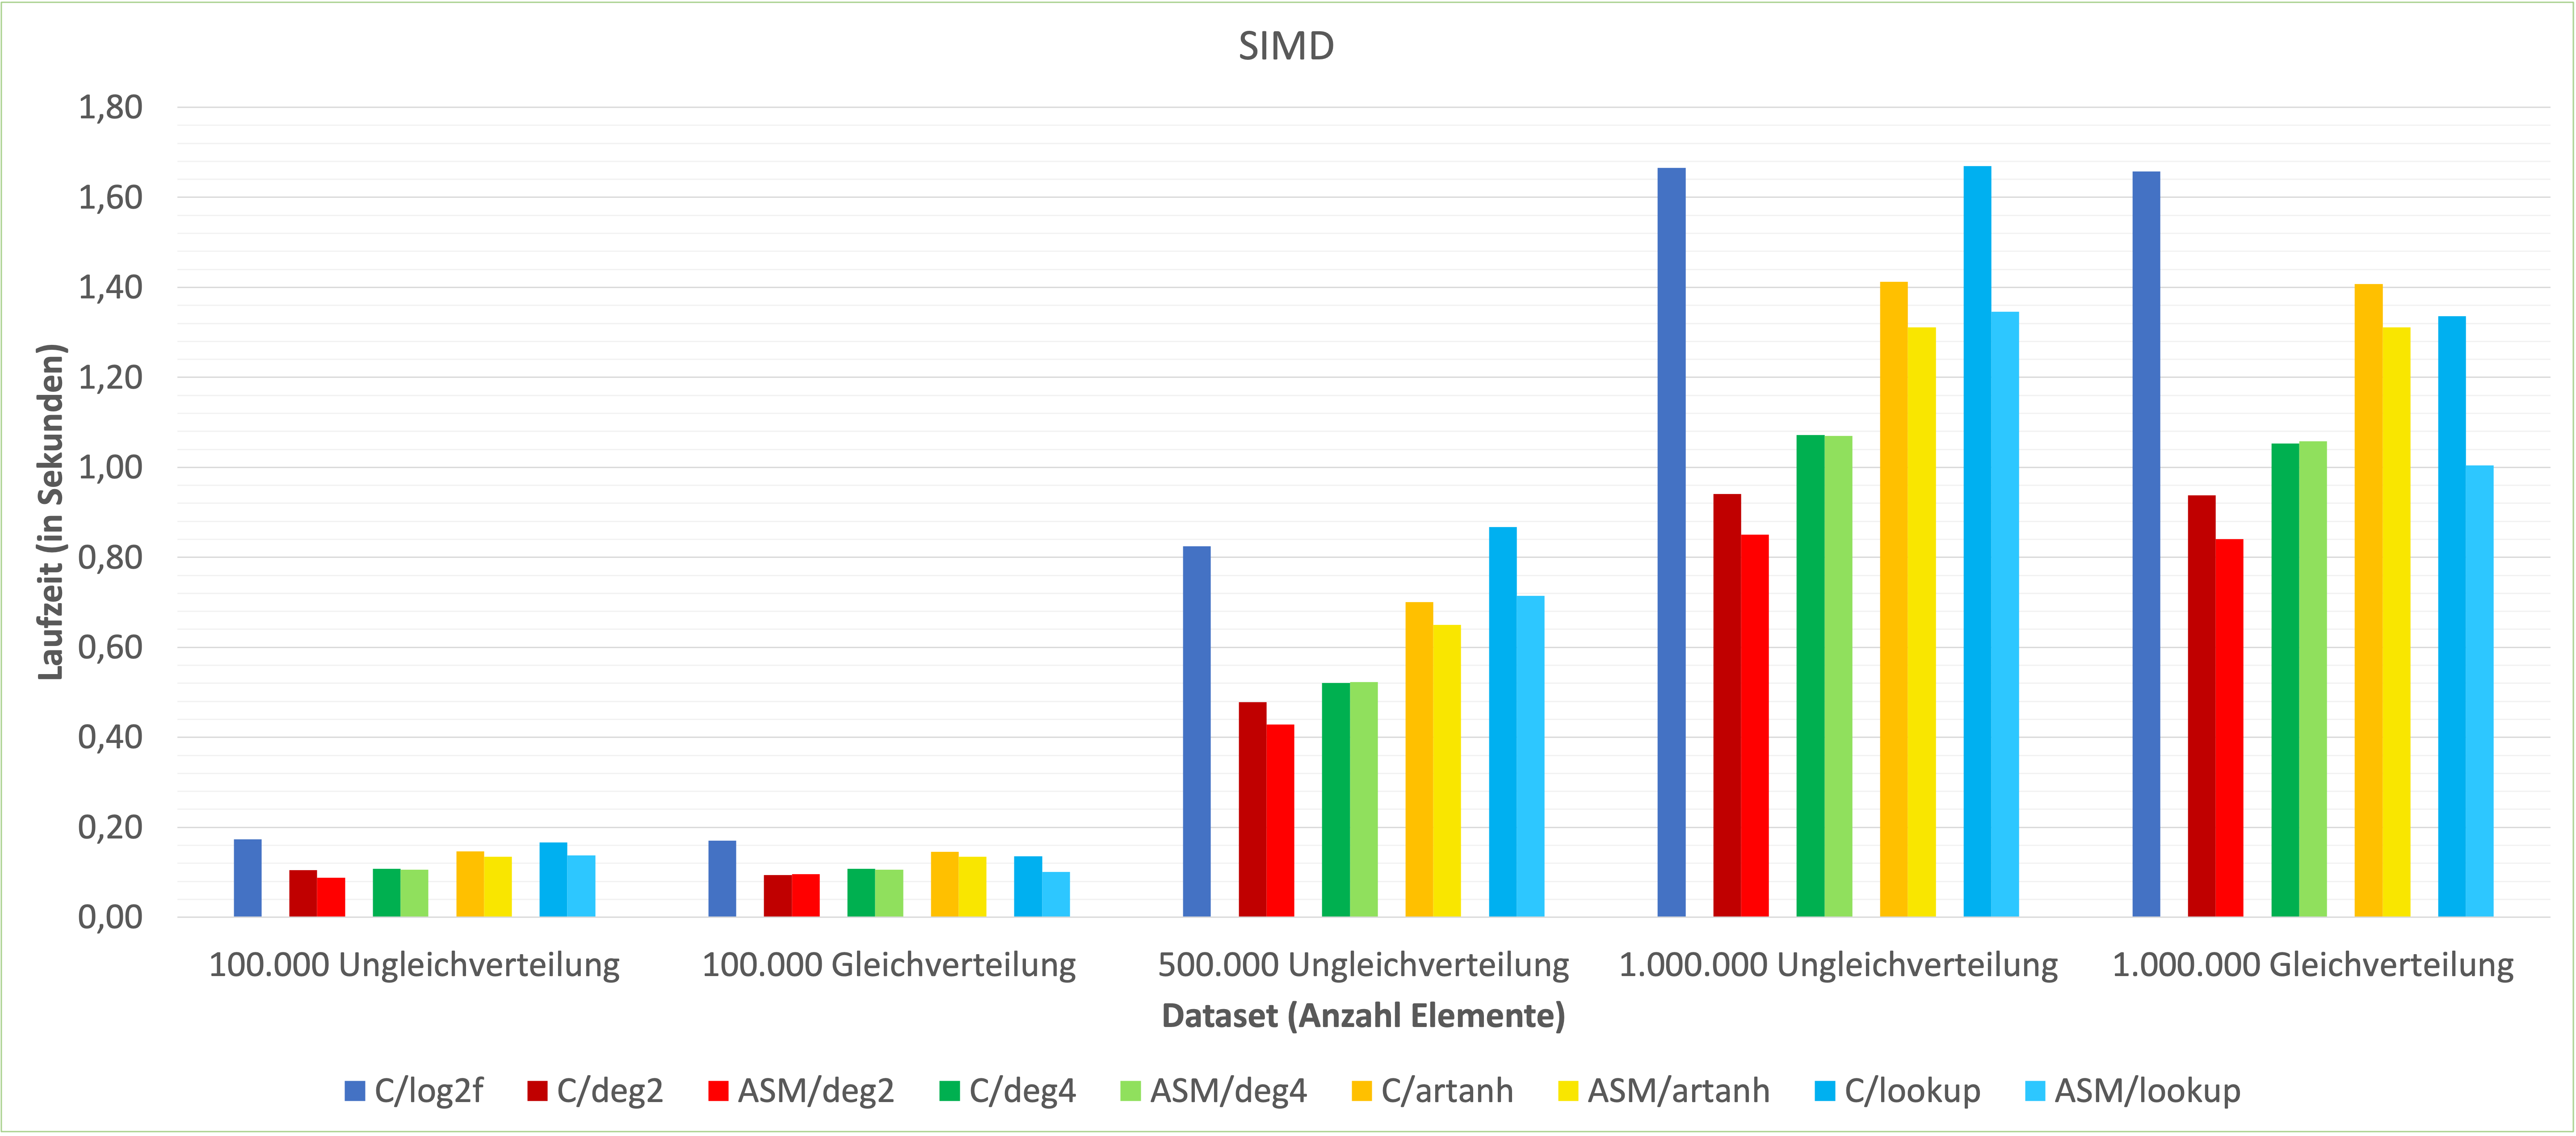
\includegraphics[scale=0.3]{graph_simd.png}
    \caption{Performazgrafik zu SIMD Implementation mit 1000 Iterationen}
    \label{fig:graph_simd}
\end{figure}

Um Grafiken zu erstellen, haben wir das Programm mit GCC 11.2 und Flag $-O3$ kompiliert und die Zeitmessungen auf Arch Linux 3.2 mit Kernel Version 5.12.8 - Intel i7-10750H @ 2.6 GHz mit $1000$ Iterationen durchgeführt.

In den Grafiken ist es zu sehen, dass unsere Logarithmusfunktionen leistungsfähiger als glibc Implementation. Darüber hinaus sind wir in der Lage, mittels Assembly unsere Funktionen noch besser als C implementieren.

Die Logarithmusfunktion mit Lookup Tabelle ist etwas schneller mit Gleichverteilungen gegen Ungleichverteilungen. Dies liegt daran, dass bei der Gleichverteilung immer der gleiche Wert von der Cache abgefragt wird.

\begin{figure}[h]
    \centering
    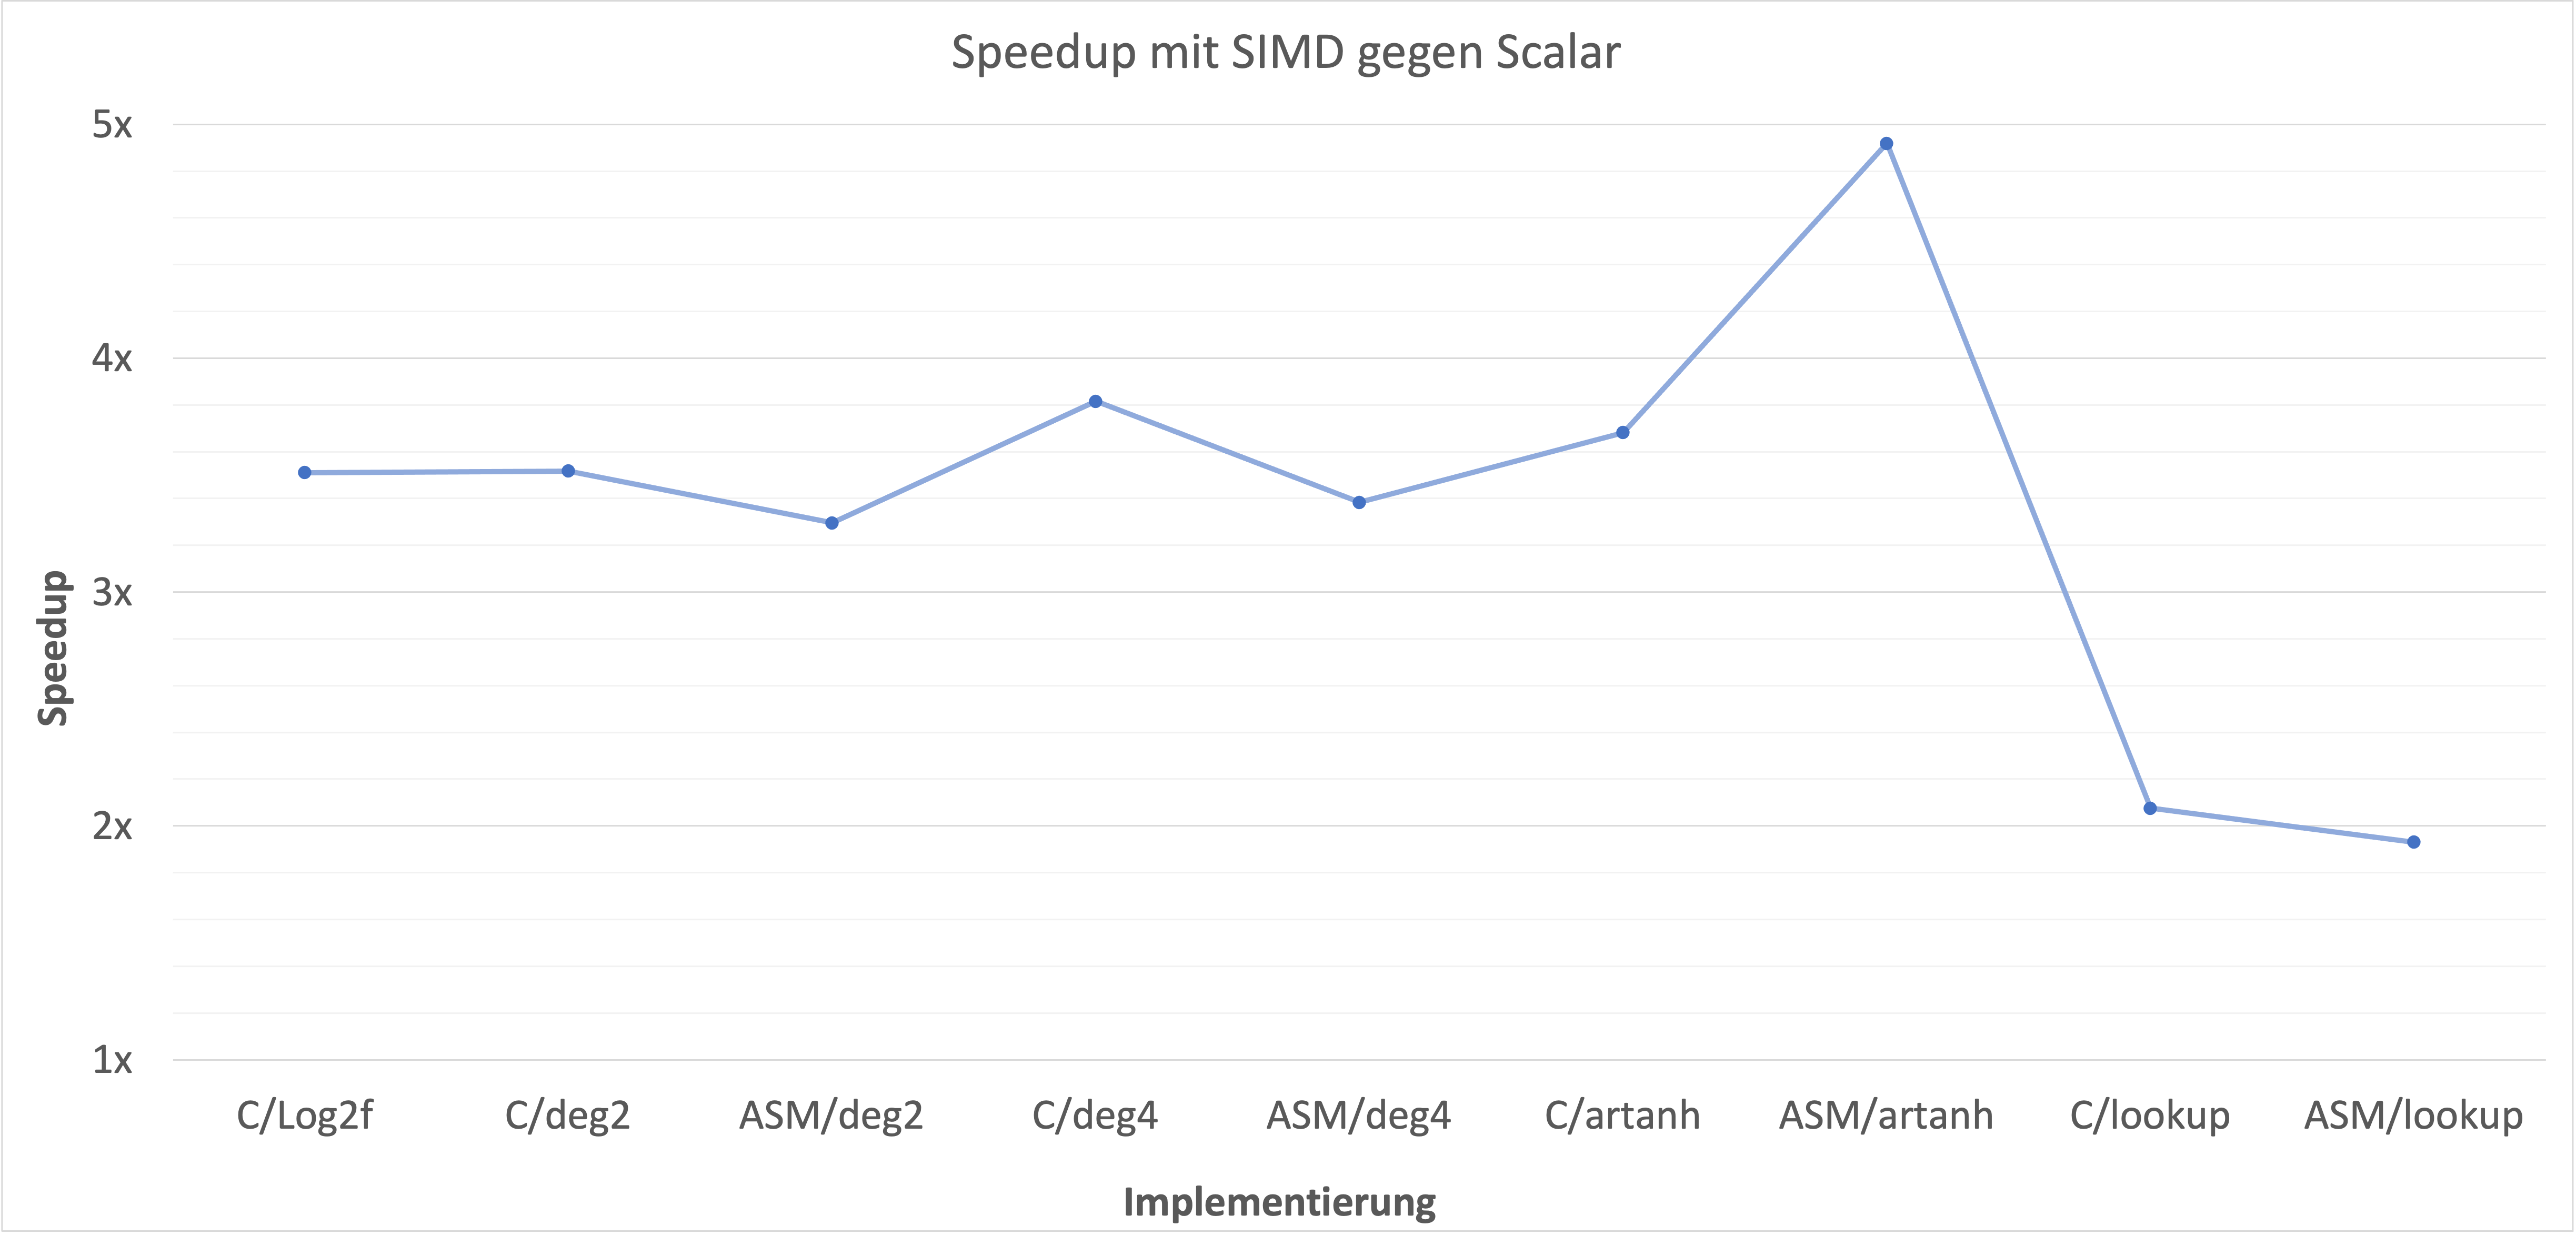
\includegraphics[scale=0.35]{graph_speedup.png}
    \caption{Speedup mit SIMD Implementation}
    \label{fig:graph_speedup}
\end{figure}

Obwohl die Glibc-Implementierung der Logarithmusfunktion ebenfalls eine Lookup-Tabelle verwendet, erreichen wir einen Speedup von $3$. Der Grund dafür ist, dass, da die Lookup Tabelle eine Größe von 16 hat, fast alle Werte immer im Cache sind. Ein weiterer Grund ist, dass wir nicht auf Sonderfälle  NaN, $\pm$Inf, $\pm$0 und negative Zahlen überprüfen, was uns einige Branches erspart.

Das durchschnittliche Speedup, das wir mittels unserer SIMD-Implementiereung außer Lookup-Tabelle ist fast $4$. Zusätzlich ist die Speedup bei der Lookup Tabelle mittels SIMD gegen Skalar fast 3 mal wegen der notwendigen Speicherzugriffe.
\section{Zusammenfassung und Ausblick}
Das Entropiefunktion wurde mit unterschiedlichen Algorithmen erfolgreich implementiert und mit einer Referenzimplementierung verglichen. Die Verwendung von Approximationen für die Logarithmusfunktion hat es uns leichter gemacht, vektorisierte Versionen unsere Algorithmen zu implementieren.

Der Einsatz von SSE-Registern und SIMD-Befehle hat für eine deutliche Performance-Steigerung gesorgt.  Was wir nicht erwartet hatten, war die Verbesserung der Genauigkeit durch die Kahans-Summe. Wir haben auch festgestellt, dass die Leistung der Assembler-Implementierung in vielen fällen deutlich besser als der C-Implementierung war.

Zusammenfassend lässt sich sagen, dass wir ASM-SIMD-DEG4 Implementierung empfehlen, da es die genaueste nach log2f und leistungsfähigste ist.

\newpage


% TODO: Fuegen Sie Ihre Quellen der Datei Ausarbeitung.bib hinzu
% Referenzieren Sie diese dann mit \cite{}.
%Beispiel: CR2 ist ein Register der x86-Architektur~\cite{intel2017man}.
\bibliographystyle{plain}
\bibliography{Ausarbeitung}{}

\end{document}
